%!TEX root =  vortrag.tex
\section{Open Data}

\frame{
\frametitle{Open Data}
\begin{definiere} [Open Data]
F�r jedermann sollte [...] ein Zugang zu jenen Daten der Verwaltung frei gegeben werden, die keinen Datenschutz-
oder Sicherheitsbeschr�nkungen unterliegen."  J�rg von Lucke in "Open Government, �ffnung von Staat und Verwaltung"
\end{definiere}}

\frame{
\frametitle{Open Data}
\begin{kasten} [Rechtsgrundlage]\begin{footnotesize}
Das "Informationsfreiheitsgesetz vom 5. September 2005 (BGBl. I S. 2722)" bildet einen juristischen Pfeiler f�r die Handhabe "offener Daten": \baselineskip \baselineskip

"� 1 Grundsatz (1) Jeder hat nach Ma�gabe dieses Gesetzes gegen�ber den Beh�rden des Bundes einen Anspruch auf Zugang zu amtlichen Informationen."\baselineskip \baselineskip

"� 2 Begriffsbestimmungen. Im Sinne dieses Gesetzes ist amtliche Information: jede amtlichen Zwecken dienende Aufzeichnung, unabh�ngig von der Art ihrer Speicherung [...]."
\end{footnotesize}\end{kasten}
\begin{kasten}
 Fehlen einer Open Data Lizenz  (wie z.B. in Gro�britannien)
\end{kasten}}

\frame{
\frametitle{Open Data}
\begin{kasten} [Grenzen]
"Wenn �ber den einzelnen B�rger Bewegungs- und Pers�nlichkeitsprofile erstellt werden oder Daten so verkn�pft werden, dass ein schwerwiegender Eingriff in die Pers�nlichkeitsrechte vorliegt, ist eine rote Linie �berschritten." - de Maiziere in einem Video auf der Seite des Innenministeriums
\end{kasten}}

\frame{
\frametitle{OpenData Network}
\begin{kasten}[OpenData Network]
Das OpenData Network propagiert die nutzbringende Verwendung offener Daten. \baselineskip \baselineskip

Grunds�tze des OpenData Networks:
	\begin{itemize}
	   \item Informationsfreiheit
	   \item B�rgerrechte in der Informationsgesellschaft
	   \item Kollaborative Formen der Partizipation
	\end{itemize}
\end{kasten}}

\frame{
\frametitle{OpenData Network}
\begin{merkmale} [OpenData Principles]
	\begin{itemize}
 	   \item Vollst�ndigkeit
 	   \item Prim�rquelle
 	   \item Zeitnah
 	   \item Zug�nglichkeit
	   \item Maschinenlesbar
	   \item Nicht diskriminierend
 	   \item Nicht propri�ter
 	   \item Lizenzfrei
	\end{itemize}
\end{merkmale}}

\frame{
\frametitle{Darstellungsformen: Dashboard}
\begin{merkmale}[Dashboard]
\begin{itemize}
  \item Visualisierung von (verteilten) Daten z.B. als Ampel-, Tachometer- oder Thermometer-Darstellung
  \item Starke Komprimierung der Informationen
  \item Informationsgehalt stark abh�ngig von Zielen und Adressaten der Visualisierung
\end{itemize}
\end{merkmale}
}

\frame{
\frametitle{Darstellungsformen: Dashboard}
\begin{figure}
\begin{center}
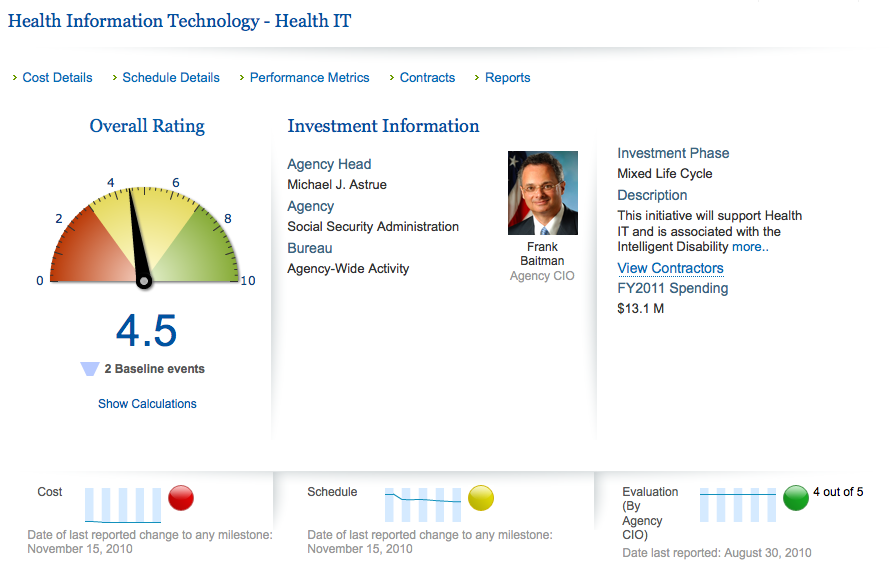
\includegraphics[width=10cm]{./images/Dashboard.png}
\end{center}
\end{figure}
}

\frame{
\frametitle{Darstellungsformen: Mashup}
\begin{merkmale}[Mashup]
\begin{itemize}
  \item Erstellung neuer Inhalte durch Kombination bereits verf�gbarer (oft �ber APIs)
  \item H�ufig Verwendung von Karten oder Darstellung von Beziehungen eines Netzwerks
  \item Meist interaktiv
\end{itemize}
\end{merkmale}
}

\frame{
\frametitle{Darstellungsformen: Mashup}
\begin{figure}
\begin{center}
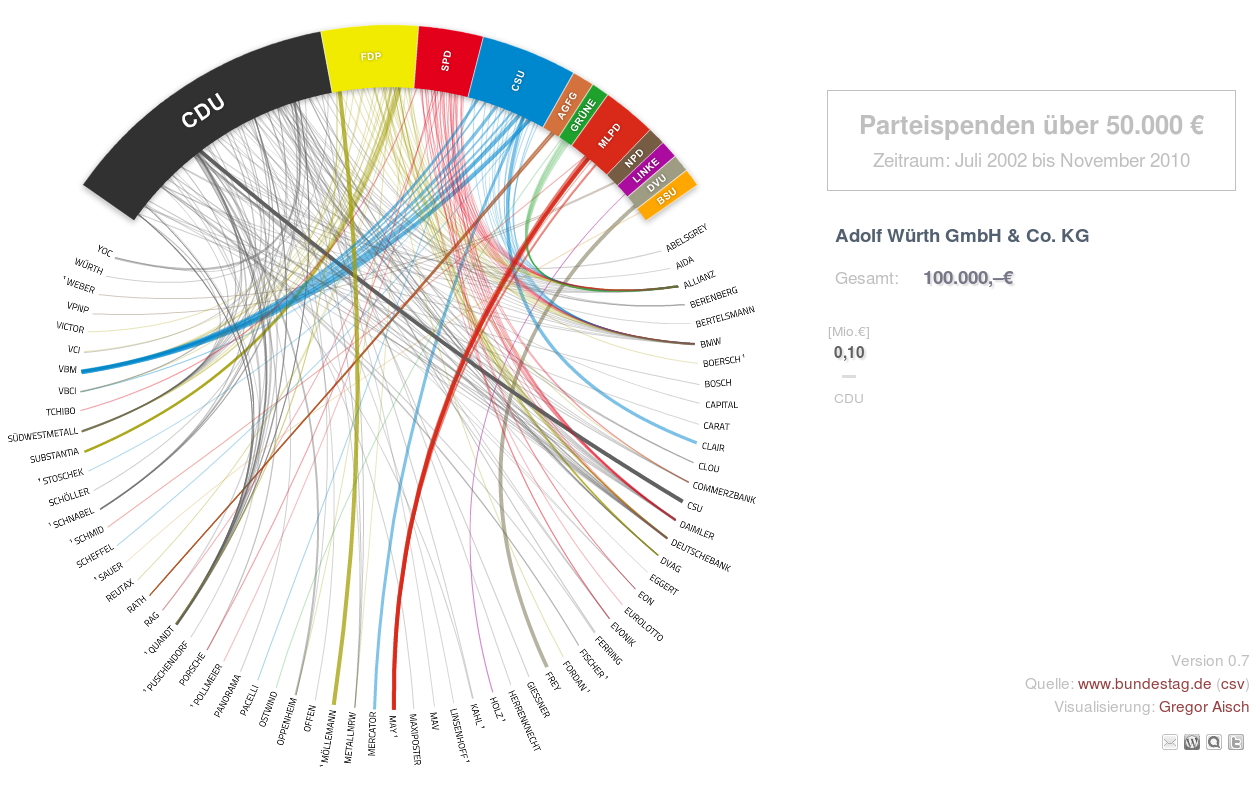
\includegraphics[width=10cm]{./images/Mashup.png}
\end{center}
\end{figure}
}

\frame{
\frametitle{Geodateninfrastruktur}
\begin{kasten}[INSPIRE Richtlinie 2004/0175]
Ziel der EU-Inspire Richtlinie 2004/0175: 

"Schaffung einer Geodateninfrastruktur in der Europ�ischen Gemeinschaft"
\end{kasten}
 \begin{merkmale}[INSPIRE]
\begin{itemize}\begin{footnotesize}
  \item Daten sollten nur einmal erhoben und vorgehalten werden
  \item Daten aus unterschiedlichen Quellen sollten miteinander kombinierbar sein
  \item Daten verschiedenen Detailgrades sollen sich nahtlos zusammenf�gen
  \item Daten sollen leicht auffindbar und transparent zur Verf�gung stehen 
\end{footnotesize}\end{itemize}
\end{merkmale}}

\frame{
\frametitle{Geodateninfastruktur}
\begin{merkmale}[Geodateninfrastruktur]
\begin{itemize}
  \item Die GDI ist ein Netzwerk zum Austausch von Geodaten zwischen Produzenten, Dienstleistern und Nutzern im Geo-Bereich und setzt die INSPIRE Richtlinie in Deutschland um
  \item Es handelt sich um eine Serviceorientierte Architektur
  \item Daten, Dienste und APIs nach ISO 191xx und Implementierungsspezifikationen des Open Geospatial Consortiums
 \end{itemize}
\end{merkmale}}

\frame{
\frametitle{Geodateninfastruktur}
\begin{merkmale}[Geodateninfrastruktur]
Ziele:
  \begin{itemize}
    \item Bessere Handlungsm�glichkeiten bei der Bek�mpfung von Umweltproblemen
    \item Zugang zu allen Geodaten, die f�r Regierungsentscheidungen notwendig sind
  \end{itemize}
\end{merkmale}}

\frame{
\frametitle{Beispiel: Offener Haushalt}
\begin{merkmale}[Offener Haushalt]
\begin{itemize}
  \item Verwendung der Rohdaten des Finanzministeriums
  \item Visuelle Aufbereitung der Daten ohne Verlust von Details durch Baumstruktur
  \item M�glichkeit der Weiterverarbeitung der Daten
\end{itemize}
\end{merkmale}}

\frame{
\frametitle{Beispiel: Offener Haushalt}
\begin{figure}
\begin{center}
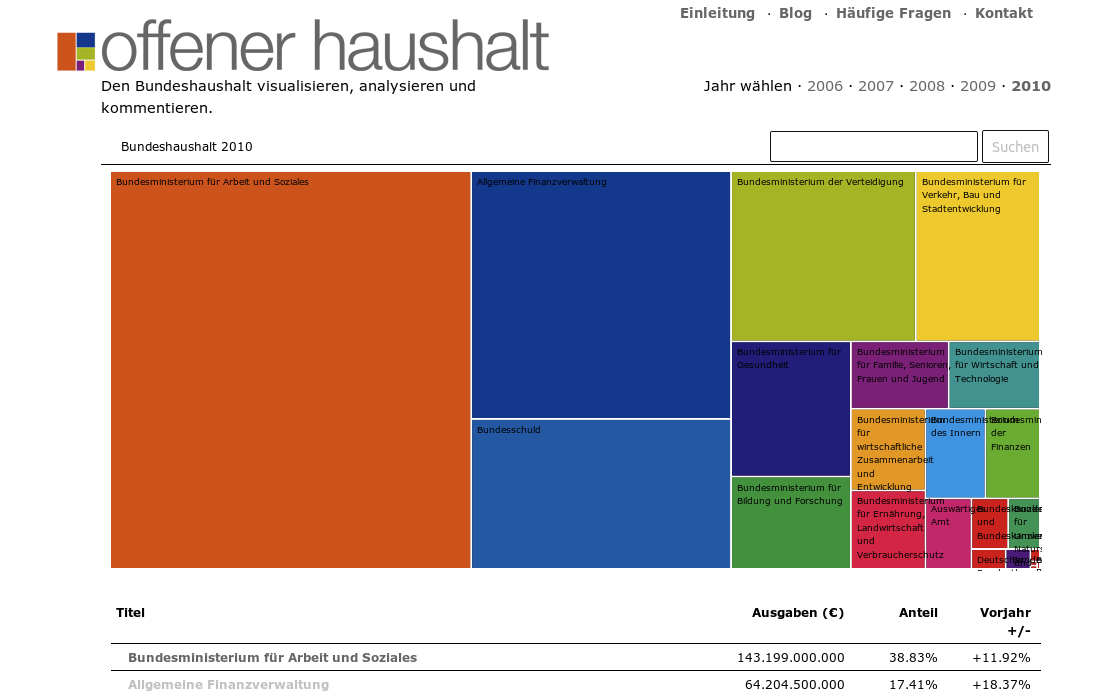
\includegraphics[width=10cm]{./images/Screen_offener_Haushalt.png}
\end{center}
\end{figure}
}

\frame{
\frametitle{Beispiel: Hackday}
\begin{definiere} [Hackday]
Hackdays sind Treffen, die das Ziel haben, zu zeigen, dass ohne gro�es Budget und in einem knappen Zeitrahmen n�tzliche Anwendungen programmiert werden k�nnen, mit denen die �ffentlichen Daten nutzbar werden.
\end{definiere}}

\frame{
\frametitle{Beispiel: Parlabla als Resultat eines Hackday}
\begin{figure}
\begin{center}
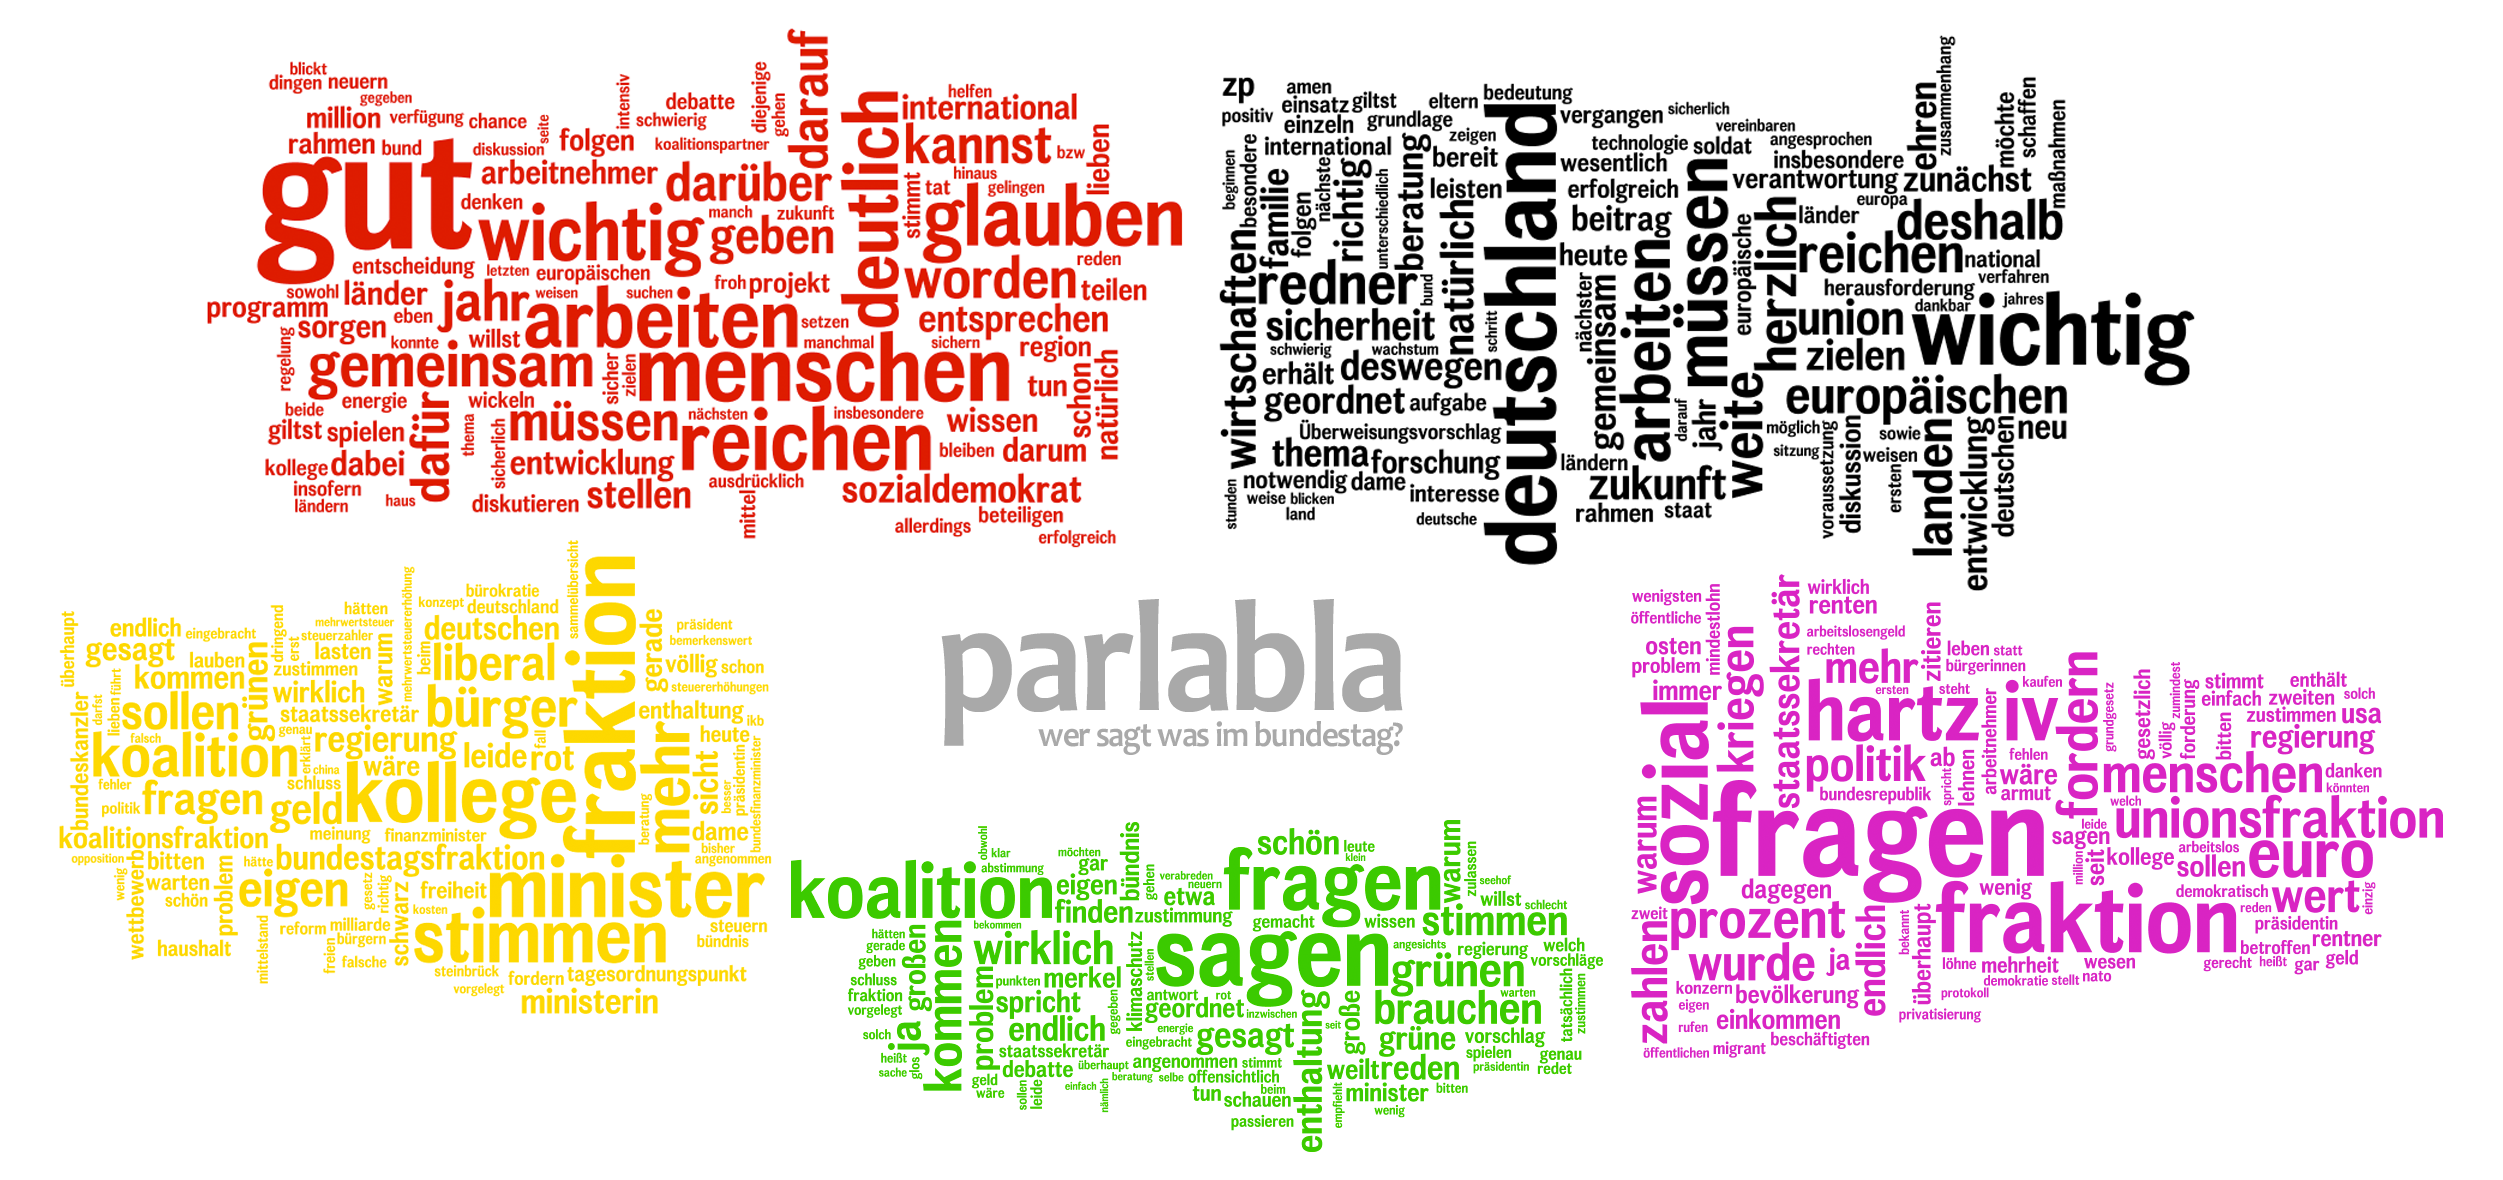
\includegraphics[width=10cm]{./images/parlabla.png}
\end{center}
\end{figure}
}